\documentclass[handout]{beamer}
\usetheme{Frankfurt}
\usefonttheme{professionalfonts}

\usepackage[utf8x]{inputenc}
\usepackage{multicol}
\usepackage{IEEEtrantools}
\usepackage{amsmath}
\usepackage{setspace}
\usepackage{subcaption}
\usepackage{pmboxdraw}
\usepackage{fancyvrb}
\setbeamertemplate{caption}[numbered]

\newcommand{\overbar}[1]{\mkern 1.5mu\overline{\mkern-1.5mu#1\mkern-1.5mu}\mkern 1.5mu}
\newcommand\Fontvi{\fontsize{9.5}{10.7}\selectfont}


\title[Development of a Coordinated Gas-Electricity optimisation model]{\normalsize{Development of a Gas-Electricity load flow and optimization model}}
\subtitle{\small{Modelling language migration and future extensions}}
\author{\texorpdfstring{Original work: }{}Allahham \& Hosseini \texorpdfstring{\\Re-coding: }{}McKinnon, Dent \& Garcia}

\institute{National Centre for Energy System Integration (CESI)}
\date{April 2020}


\subject{Optimisation in Power Models}

\begin{document}

\begin{frame}
  \titlepage
\end{frame}

\begin{frame}{Outline}
  \tableofcontents
  % You might wish to add the option [pausesections]
\end{frame}

%%%%%%%%%%%%%%%%%%%%%%%%%%%%%%%%%%%%%%%%%%%%%%%%%%%%%%%%%%%%%%%%%%%%%%%%%%%%%%%%%%%%%%%%%%%%%%
%%%%%%%%%%%%%%%%%%%%%%%%%%%%%%%%%%%%%%%%%%%%%%%%%%%%%%%%%%%%%%%%%%%%%%%%%%%%%%%%%%%%%%%%%%%%%%

\section{Goal}

\begin{frame}[t]{Goal}

  CESI is a multi-discipline knowledge and skill centre with topics and discussions crossing multiple fields, where easy-to-access tools are fundamental to enable these discussions.\\[12pt]

  While the existing optimisation models and implementations work well within their current scope, we see advantages in coding the models using a modelling language.
  
  Note load flow models may be formulated as optimization models with constant objectives.

  \begin{figure}
  \begin{center}
  
\includegraphics[width=.60\textwidth]{CESI.png}
  \end{center}
  \end{figure}

\end{frame}


%%%%%%%%%%%%%%%%%%%%%%%%%%%%%%%%%%%%%%%%%%%%%%%%%%%%%%%%%%%%%%%%%%%%%%%%%%%%%%%%%%%%%%%%%%%%%%

\begin{frame}[t]{Goal (cont.)}
  \vspace{0.5cm}
  The benefits we see in using a modelling language are:\\[12pt]

  \begin{enumerate}
    \item To provide a robust framework for easily extendable models using Allahham \& Hosseini as a base.
    \item To facilitate access to the tools by using open-source software.
    \item To enable end-users to easily modify and/or adapt the models according to their needs.
    \item To benefit from the use of mature optimisation solvers potentially speeding up the solution of models.
    \item To be able to model and solve different forms of problems, e.g. models with integer decisions.
    \item To allow for different data sets to be easily integrated into the models.
  \end{enumerate}

\end{frame}


%%%%%%%%%%%%%%%%%%%%%%%%%%%%%%%%%%%%%%%%%%%%%%%%%%%%%%%%%%%%%%%%%%%%%%%%%%%%%%%%%%%%%%%%%%%%%%
%%%%%%%%%%%%%%%%%%%%%%%%%%%%%%%%%%%%%%%%%%%%%%%%%%%%%%%%%%%%%%%%%%%%%%%%%%%%%%%%%%%%%%%%%%%%%%

\section{Introduction}

\subsection*{Optimisation models}

\begin{frame}[t]{What is a computer model}
  \vspace{0.5cm}
  Four components:\\[12pt]

  \begin{enumerate}
    \item Model specification / governing equations / other synonyms -- this is something which would be specified on paper, and exists independently of any particular data or computer implementation.
    \item Data for specific cases.
    \item (Possibly) a numerical scheme to evaluate outputs (in some cases direct solution is possible but not here). Again this exists independently of specific data or computer implementation, and is something specified on paper.
    \item Computer implementation.
  \end{enumerate}

\end{frame}


%%%%%%%%%%%%%%%%%%%%%%%%%%%%%%%%%%%%%%%%%%%%%%%%%%%%%%%%%%%%%%%%%%%%%%%%%%%%%%%%%%%%%%%%%%%%%%

\begin{frame}[t]{Introduction}{Optimisation models}
\textbf{What is an optimisation model?}\\[6pt]

Finding the best available solution to a problem subject to certain constraints on values variables can take. \\[6pt]

An optimization model has three components:
\begin{enumerate}
  \item An objective function. This is the function that needs to be optimised (maximised or minimised).
  \item Decision variables. The variables in the mathematical problem that can be varied; the aim is to find the combination of variables which gives the `best' value of the objective function.
  \item Constraints on the decision variables. These are usually expressed as equality or inequality constraints on functions of the decision variables.
\end{enumerate}
\end{frame}

%%%%%%%%%%%%%%%%%%%%%%%%%%%%%%%%%%%%%%%%%%%%%%%%%%%%%%%%%%%%%%%%%%%%%%%%%%%%%%%%%%%%%%%%%%%%%%

\begin{frame}{Introduction}{Optimisation models (cont.)}
\textbf{What is an optimisation model?}\\[6pt]

\begin{block}{Objective function}
\vspace{-0.4cm}
  \begin{IEEEeqnarray*}{c}
    \min_{x} \quad f(x)
  \end{IEEEeqnarray*}
\end{block}

\begin{block}{Contraints}
subject to:
\vspace{-0.8cm}
\begin{IEEEeqnarray*}{rcl}
  g(x)&\;=\;&0\\
  h(x) &\;\leq\;& 0\\
  x &\;\geq\;& 0
\end{IEEEeqnarray*}

\end{block}

\begin{block}{Variables and Data}
\begin{itemize}
  \item Variables. $x \in \mathbb{R}^n$ (or subset thereof)
%  \item Data. Encoded in $f$, $g$ and $h$.
\end{itemize}
\end{block}


\end{frame}

%%%%%%%%%%%%%%%%%%%%%%%%%%%%%%%%%%%%%%%%%%%%%%%%%%%%%%%%%%%%%%%%%%%%%%%%%%%%%%%%%%%%%%%%%%%%%%

\begin{frame}[t]{Introduction}{Example: Economic dispatch with energy limits}
\Fontvi
\textbf{Description:}\\
Minimise the total cost of generation in a day, by satisfying the power demand while using optimally generators G1, G2 and G3; where G1 is limited in the energy it can produce.\\[6pt]

\textbf{Sets:}
\begin{itemize}
    \item {\makebox[0.75cm]{$\mathcal{G}$\hfill}: Set of generators. Here $\mathcal{G} = \{G1,G2,G3\}$}
    \item {\makebox[0.75cm]{$\mathcal{G}^E$\hfill}: Subset of generators with energy limits. $\mathcal{G}^E = \{G1\}$}
    \item {\makebox[0.75cm]{$\mathcal{T}$\hfill}: Set of periods or hours in a day. $\mathcal{T} = \{1,2...24\}$}
\end{itemize}

\textbf{Parameters:}
\begin{itemize}
    \item {\makebox[0.75cm]{$P^D_t$\hfill}: Power demand in period $t$}
    \item {\makebox[0.75cm]{$\overbar{P}_g$\hfill}: Maximum power output of generator $g$}
    \item {\makebox[0.75cm]{$U_g$\hfill}: Total energy available from generator $g$}
    \item {\makebox[0.75cm]{$C^G_g$\hfill}: Energy price (£/MWh) of generator $g$}
\end{itemize}

\textbf{Variables:}
\begin{itemize}
    \item {\makebox[0.75cm]{$p^G_{gt}$\hfill}: Power output of generator $g$ in period $t$}
\end{itemize}
\end{frame}

%%%%%%%%%%%%%%%%%%%%%%%%%%%%%%%%%%%%%%%%%%%%%%%%%%%%%%%%%%%%%%%%%%%%%%%%%%%%%%%%%%%%%%%%%%%%%%

\begin{frame}[t]{Introduction}{Example: Economic dispatch with energy limits (cont.)}
\textbf{Objective:}\\
$$\min \quad \sum_{g \in \mathcal{G}} C^G_g \; \sum_{t \in \mathcal{T}} p^G_{gt}$$
\textbf{Constraints:}\\
\begin{IEEEeqnarray*}{rcl}
\text{Power balance: } \quad & \sum_{g \in \mathcal{G}} p^G_{gt} = P^D_t & \quad \forall t \in \mathcal{T}\\
\text{Energy consumption limits: } \quad &  \sum_{t \in \mathcal{T}} p^G_{gt} \leq U_g & \quad \forall g \in \mathcal{G}^E \\
\text{Generator limits: } \quad & 0 \leq p^G_{gt} \leq \overbar{P}_g & \quad \forall g \in \mathcal{G}, t \in \mathcal{T}
\end{IEEEeqnarray*}

\textbf{Note:}
Not yet specified anything about a specific instance, including the size of the sets

\end{frame}

%%%%%%%%%%%%%%%%%%%%%%%%%%%%%%%%%%%%%%%%%%%%%%%%%%%%%%%%%%%%%%%%%%%%%%%%%%%%%%%%%%%%%%%%%%%%%%

\begin{frame}[t]{Introduction}{Optimisation models (cont.)}

The form of the objective function together with the constraints and nature of the variables will determine the type of problem to be solved.\\[12pt]

Some examples of types of problem:\\[12pt]
\begin{itemize}
\item Linear programming: $f$,$g$ and $h$ are linear.
\item (Mixed) Integer programming: integer solution required (for some variables).
\item Non-linear programming: $f$ or $g$ or $h$ are non-linear.
\end{itemize}

\end{frame}

%%%%%%%%%%%%%%%%%%%%%%%%%%%%%%%%%%%%%%%%%%%%%%%%%%%%%%%%%%%%%%%%%%%%%%%%%%%%%%%%%%%%%%%%%%%%%%



\section{Programming languages and software}

\begin{frame}[t]{Programming languages and software}
  In order to solve problems ranging from a couple to potentially hundreds of thousands variables with complex constraints we need to code the models in computer languages.\\[12pt]

  For optimisation problems, we need to decide 
  
  the software tools used might be divided  into 3 main categories:
  \begin{enumerate}
    \item What we will code, and what we will use pre-built tools for
    \item What language do we use
  \end{enumerate}

  Environments can be divided into
  \begin{enumerate}
    \item General-purpose programming languages
    \item Specialist mathematical languages
    \item Algebraic modelling languages
  \end{enumerate}

\end{frame}

%%%%%%%%%%%%%%%%%%%%%%%%%%%%%%%%%%%%%%%%%%%%%%%%%%%%%%%%%%%%%%%%%%%%%%%%%%%%%%%%%%%%%%%%%%%%%%


\subsection{General purpose languages}
\begin{frame}{Programming languages and software}{General-purpose programming languages}
\textbf{General-purpose programming languages} are designed to be used for writing software in the widest variety of application domains. Thus they lack highly specialized features for a particular domain such as optimisation, though are flexible in the range of tasks to be performed, and often permit very efficient code.\\[6pt]

Examples: C++, Fortran, Visual Basic, Java, Python, \underline{Julia}.\\[12pt]

\begin{figure}
\begin{center}

\includegraphics[width=.60\textwidth]{GeneralLang.png}
\end{center}
\end{figure}

\end{frame}

%%%%%%%%%%%%%%%%%%%%%%%%%%%%%%%%%%%%%%%%%%%%%%%%%%%%%%%%%%%%%%%%%%%%%%%%%%%%%%%%%%%%%%%%%%%%%%

\begin{frame}{Programming languages and software}{General-purpose programming languages}
\textbf{Mathematical programming languages} are similar to general-purpose languages in the sense that they cover a broad range of applications, but they have been developed to be efficient with certain mathematical aspects (either specifying problems or computation). \\[6pt]

Examples:

\begin{itemize}
  \item Numerical calculations: Matlab, R and \underline{Julia}.
  \item Symbolic algebra: Mathematica and Maple.
\end{itemize}


\begin{figure}
\begin{center}

\includegraphics[width=.60\textwidth]{MathLang.png}
\end{center}
\end{figure}

\end{frame}

%%%%%%%%%%%%%%%%%%%%%%%%%%%%%%%%%%%%%%%%%%%%%%%%%%%%%%%%%%%%%%%%%%%%%%%%%%%%%%%%%%%%%%%%%%%%%%

\subsection{Algebraic modelling languages}
\begin{frame}[t]{Programming languages and software}{Algebraic modelling languages}
\textbf{Algebraic modelling languages} are computer programming languages which allow specification of optimization problems in the same form as on paper, combining this with data to create a specific instance (or generated mathematical program, etc), and pass it to a solver. For nonlinear programs automatic differentiation of objective and constraint functions is provded.\\[6pt]

For specifying problems there is no programming in the traditional sense; there may be a scripting language. Language elements include sets, indices, algebraic expressions, index and data handling.\\[6pt]

Examples: AMPL, AIMMS, GAMS, Lindo, JuMP\footnote[frame]{Modelling language extension for Julia.}.

\begin{figure}
\begin{center}

\includegraphics[width=.40\textwidth]{AML.png}
\end{center}
\end{figure}


\end{frame}

%%%%%%%%%%%%%%%%%%%%%%%%%%%%%%%%%%%%%%%%%%%%%%%%%%%%%%%%%%%%%%%%%%%%%%%%%%%%%%%%%%%%%%%%%%%%%%

\begin{frame}[t,fragile]{Programming languages and software}{Example syntax in JuMP (Algebraic modelling)}
\begin{itemize}
\item Constraint for Power Generation Limits:
\begin{itemize}
  \item Expression:
  $$P^{LB}_g \leq p_{g,t} \leq  P^{UB}_g \quad \forall g \in \mathcal{G},\; \forall t \in \mathcal{T}$$\\
  \item Code:
  \hspace{-1.5cm}\begin{Verbatim}[fontsize=\scriptsize]
    @constraint(m, PLim[g ∈ G, t ∈ T], P_LB[g] ≤ p[g,t] ≤ P_UB[g])
  \end{Verbatim}
\end{itemize}\vspace{12pt}
\item Objective function:
\begin{itemize}
  \item Expression:
  $$\min \quad \sum_{g \in \mathcal{G}} C_g \sum_{t \in \mathcal{T}} p_{g,t}$$\\
  \item Code:
  \hspace{-1.5cm}\begin{Verbatim}[fontsize=\scriptsize]
    @objective(m, Min, ∑(C[g]*∑(p[g,t] for t ∈ T) for g ∈ G))
  \end{Verbatim}
\end{itemize}

\end{itemize}

\end{frame}

%%%%%%%%%%%%%%%%%%%%%%%%%%%%%%%%%%%%%%%%%%%%%%%%%%%%%%%%%%%%%%%%%%%%%%%%%%%%%%%%%%%%%%%%%%%%%%

\subsection{Solvers}
\begin{frame}{Programming languages and software}{Solvers}
A \textbf{solver} is a software tool which identifies the optimal solution for a specific instance of an optimization problem.
Commonly a solver is for a specific class of problem (LP, MILP, NLP, etc).\\[6pt]

Necessary to pass to the solver:
\begin{itemize}
    \item LP: Constraint matrix, and objective fn and RHS vectors
    \item NLP: Constraint and objective fns, (plus 1st/2nd derivatives either in modelling language or solver)
\end{itemize}

Examples: CPLEX (LP, MILP, SDP, SOCP), Gurobi (LP, MILP SDP, SOCP), Knitro (MINLP), Ipopt (NLP).

\begin{figure}
\begin{center}

\includegraphics[width=.75\textwidth]{Solvers.png}
\end{center}
\end{figure}



\end{frame}

%%%%%%%%%%%%%%%%%%%%%%%%%%%%%%%%%%%%%%%%%%%%%%%%%%%%%%%%%%%%%%%%%%%%%%%%%%%%%%%%%%%%%%%%%%%%%%

\begin{frame}[t]{Programming languages and software}{Proposal (cont.)}
  \begin{figure}
  \begin{center}
  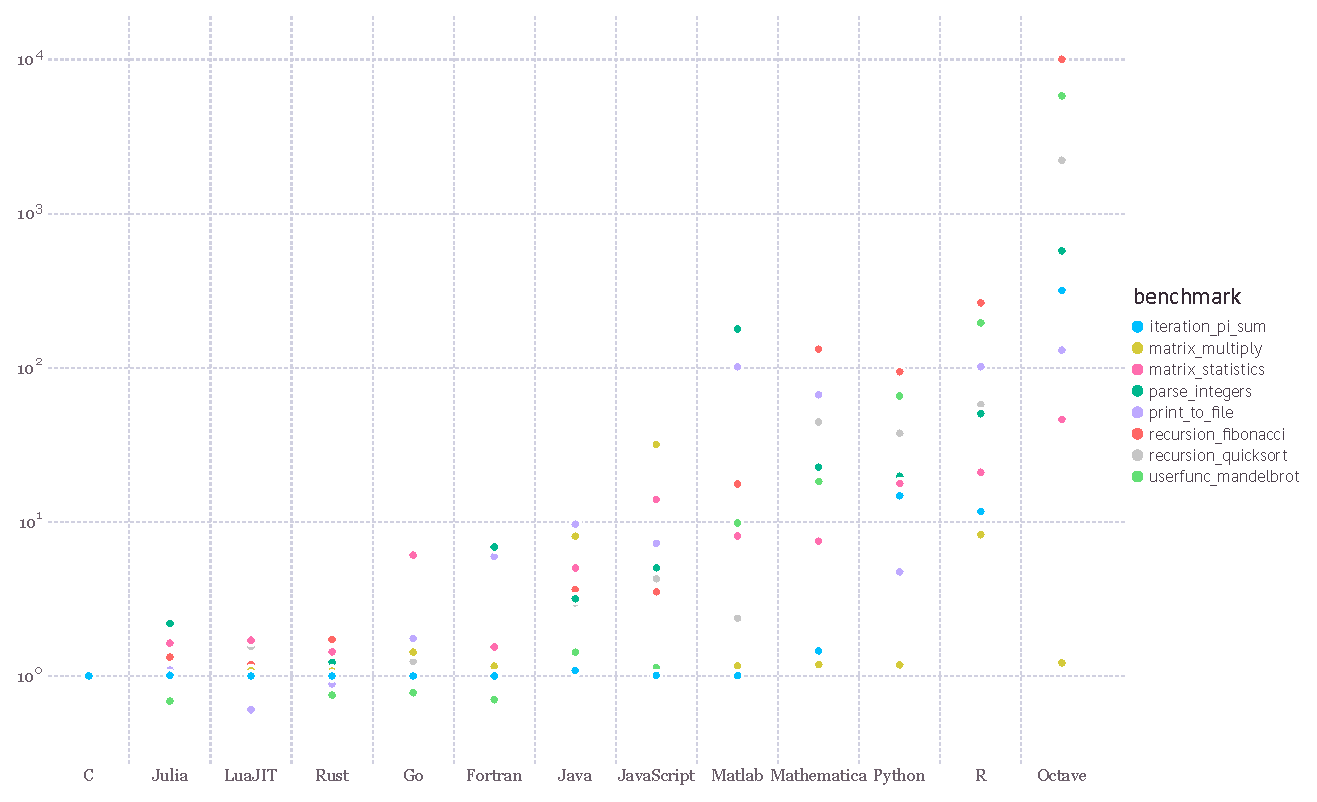
\includegraphics[width=0.95\textwidth]{benchmarks.eps}
  \end{center}
  \caption{Benchmark of some common programming languages}\label{fig:speed}
  \end{figure}

\end{frame}

%%%%%%%%%%%%%%%%%%%%%%%%%%%%%%%%%%%%%%%%%%%%%%%%%%%%%%%%%%%%%%%%%%%%%%%%%%%%%%%%%%%%%%%%%%%%%%

\begin{frame}[t]{What lies behind our proposal}

\textbf{Resusable on different datasets/examples}.\\[6pt]

\textbf{Low development time}. Quick transfer of paper-based model in computer environmnent.\\[6pt]

\textbf{Easily extensible}. i.e. adding different constraints, time element, optimization versus load flow, etc.\\[6pt]

\textbf{Automated combination of model and data, and differentiation}. It is not nice to hard code any of this for specific cases.\\[6pt]

\textbf{Use efficient general purpose solvers}. Don't want to think about solution algorithm, typically no benefit in doing so unless exploiting block structure in constraint matrix.

\end{frame}


%%%%%%%%%%%%%%%%%%%%%%%%%%%%%%%%%%%%%%%%%%%%%%%%%%%%%%%%%%%%%%%%%%%%%%%%%%%%%%%%%%%%%%%%%%%%%%


\subsection{Proposal}
\begin{frame}[t]{Programming languages and software}{Proposal}
  To use and integrated programming approach by incorporating into our modelling and solving approaches the 3 main softare elements used for optimisation. This allows for flexibility, robustness and speed. In concrete to:\\[12pt]
\begin{enumerate}
  \item Use \textbf{Julia} as a general/mathematical progamming software.
  \item Use \textbf{JuMP} as a algebraic modelling language.
  \item Use a solver (\textbf{Ipopt} or others).
\end{enumerate}
\end{frame}

\begin{frame}[t]{Programming languages and software}{Proposal (cont.)}
  \textbf{Why?}\\[12pt]
  Julia is free, fast (Figure \ref{fig:speed}) and has a friendly syntax (similar to Matlab). Julia has had an important increase of optimisation users that benefit from the tight integration with JuMP. Julia is compatible with other languages and have packages to integrate it with other languages such as Python.\\[6pt]

  JuMP is also free, fast and friendly. It benefits from being solver-agnostic and benchmarking has shown that can create problems at similar speeds than AMPL.
\end{frame}

\begin{frame}[t]{Programming languages and software}{Proposal (cont.)}
  \begin{figure}
  \begin{center}
  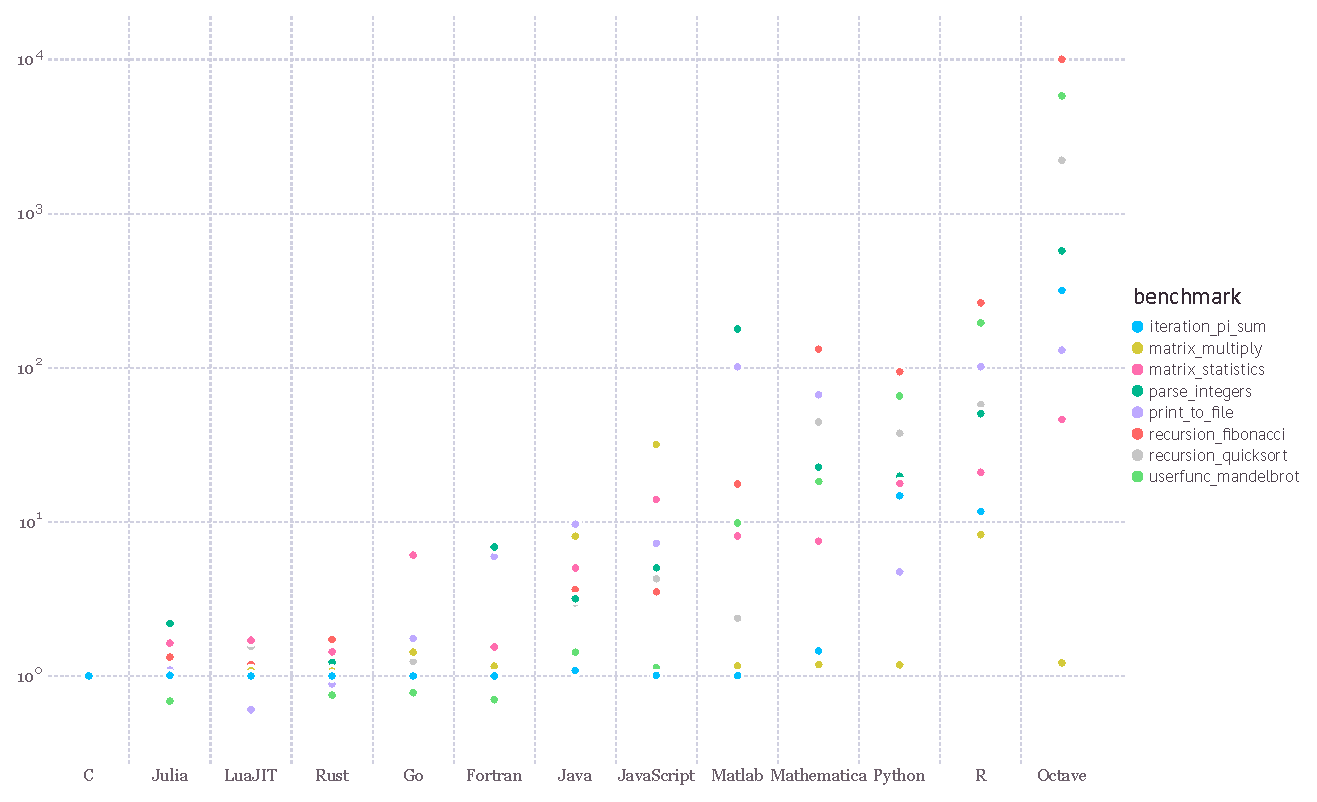
\includegraphics[width=0.95\textwidth]{benchmarks.eps}
  \end{center}
  \caption{Benchmark of some common programming languages}\label{fig:speed}
  \end{figure}

\end{frame}

\section{Modelling components}

\subsection{Model}
\begin{frame}[t]{Modelling components}{Model}

  The optimisation \textbf{model} considers the whole set of equations that define the behaviour and response of a system. The model once written in an algebraic way can be then ''coded" in the algebraic software (JuMP).\\[6pt]

  If new components of the system are considered or the dynamics change, then the model needs to be modified to reflect this situation. Examples of modifications of the model in this context are: extensions to multi-period operational problems, capacity planning problems, heat-network integrations, etcetera.
\end{frame}

\subsection{Data}
\begin{frame}[t]{Modelling components}{Data}
  The same dynamics in a system (model) can behave differently depending on the \textbf{Data}. The data needs to be read and integrated as parameters in the model. The data can come from different datasets and have information of different places. Such as information about Findhorn or Newcastle.\\[6pt]

  There are many different ways of reading data into Julia, directly or with the use of diverse packages and formats. It is important to mention that standard matpower formats are limited in their reach, as they cannot easily handle multi-period settings or other extensions.

\end{frame}


\section{Re-coding implementation}

\subsection{Progress}
\begin{frame}[t]{Re-coding}{Activities}

The aim of this work is to use Allahham \& Hosseini gas-electricity optimsiation model and recoding it to benefit from the use of Julia, JuMP and solvers (for the reasons stated before). \\[12pt]

Also, McKinnon has done a recoding in AMPL that shares most of the benefits of the Julia/JuMP recode.

\end{frame}

\begin{frame}[t]{Re-coding}{Progress}

Progress to date:
\begin{itemize}
  \item Read the full code, analysed how the data and model are linked and what were the implications of extending this code to more general cases.
  \item Developed an integrated data management module for reading and writing friendly datafiles, without the need of external packages. We've chosen to use a clean and robust ''format" based on the AMPL data formats for the electrical networks, gas networks and the coupling nodes.
  \item Coded routines for matpower data file reading, so standard matpower cases can be easily used, without the need of Matlab or manual conversions of the data files.
  \item Verified cases between re-codings Matlab-AMPL-Julia
\end{itemize}

\end{frame}

\begin{frame}[t]{Re-coding}{Data}
At the moment, the data can be read easily in matpower format or in the AMPL-like format. Here are snapshots of both formats.

\begin{figure}
\begin{center}
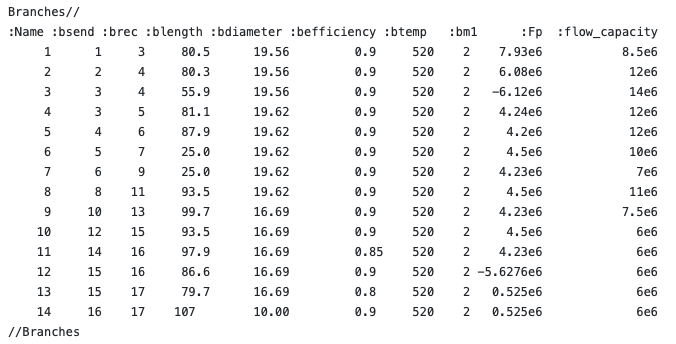
\includegraphics[height=0.55\textheight]{AMPLlike2.png}
\end{center}
\caption{AMPL-like data format}\label{fig:ampllike}
\end{figure}
\end{frame}


\begin{frame}{Re-coding}{Data (cont.)}

\begin{figure}
\begin{center}
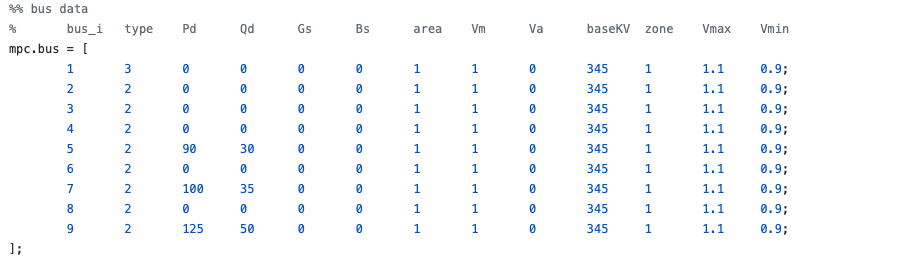
\includegraphics[width=\textwidth]{Matpowerlike2.png}
\end{center}
\caption{Matpower-like data format}\label{fig:matpowerlike}
\end{figure}


\end{frame}

\subsection*{Models}

\begin{frame}[t]{Re-coding}{Models}

  The models are written in JuMP and consist in roughly 3 groups of equations. The first group consist in capturing the physics and limitations of the electrical network (in A\&H integrated model, they rely on the model specified in matpower), the physics of the gas networks (specified by A\&H in their own equations) and finally, the links between networks.\\[6pt]

  The problem is then solved using interior point methods by the solver (Ipopt) without the need of manually specifying and creating vectors with derivatives (Jacobians) or any other symbolic or numerical routine. All is done efficiently by the solver.
\end{frame}

\begin{frame}[t]{Re-coding}{Models (cont.)}
  An extract of the electrical model can be seen here:

  \begin{figure}
  \begin{center}
  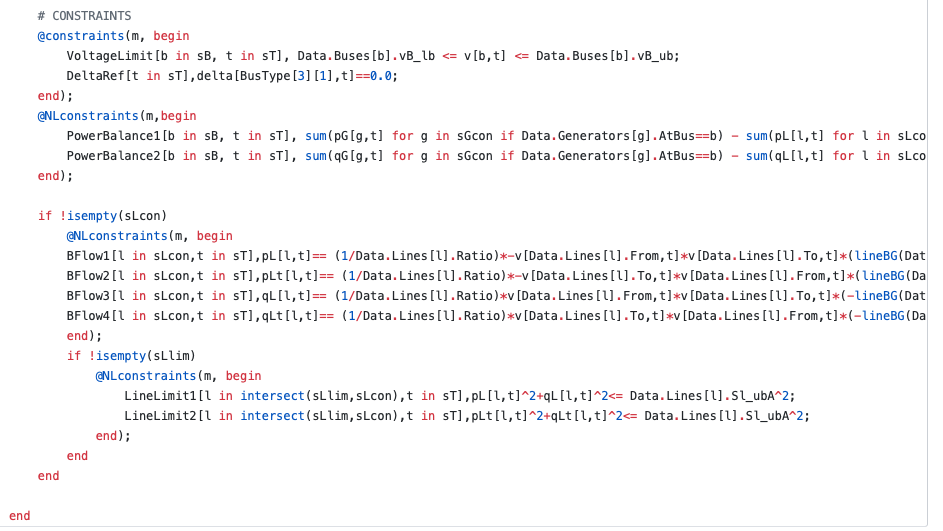
\includegraphics[height=0.55\textheight]{OPF2.png}
  \end{center}
  \caption{Electrical network constraints (extract)}\label{fig:opf}
  \end{figure}

\end{frame}


\subsection{Demonstration}

  \begin{frame}{Re-coding}{Demonstration}
    \textbf{Live walktrough the code and its execution}\\[12pt]
    (Show Julia/JuMP code vs. original code to show the dramatic difference in complexity)
  \end{frame}

\subsection{Discussion}
\begin{frame}{Re-coding}{Discussion}
  \textbf{How can be used and what is needed to take it forward?}\\[12pt]
  (Discussion by Chris, ask him for some points here.)

\end{frame}

\end{document}
